\chapter{Introduction}
\label{ch:chapter_one}

This thesis opens with an introduction to the research background, followed by an overview of unmanned systems and their deployment in this context. Considering current advancements in robotics, the main topic of this work is then introduced, along with its motivation, objectives, and workflow. Finally, a summary of the upcoming chapters is provided.

\section{Background}
\label{sec:background}

Exploration, collection of samples, environmental monitoring, disaster response, and infrastructure inspection. 
Those activities have one problem in common, they take place in highly unpredictable environments, sometimes unreachable or too dangerous for humans. Here, chaos reigns, and deploying autonomous systems is as inevitable as it is complex. 

\begin{figure}[H]
    \centering
    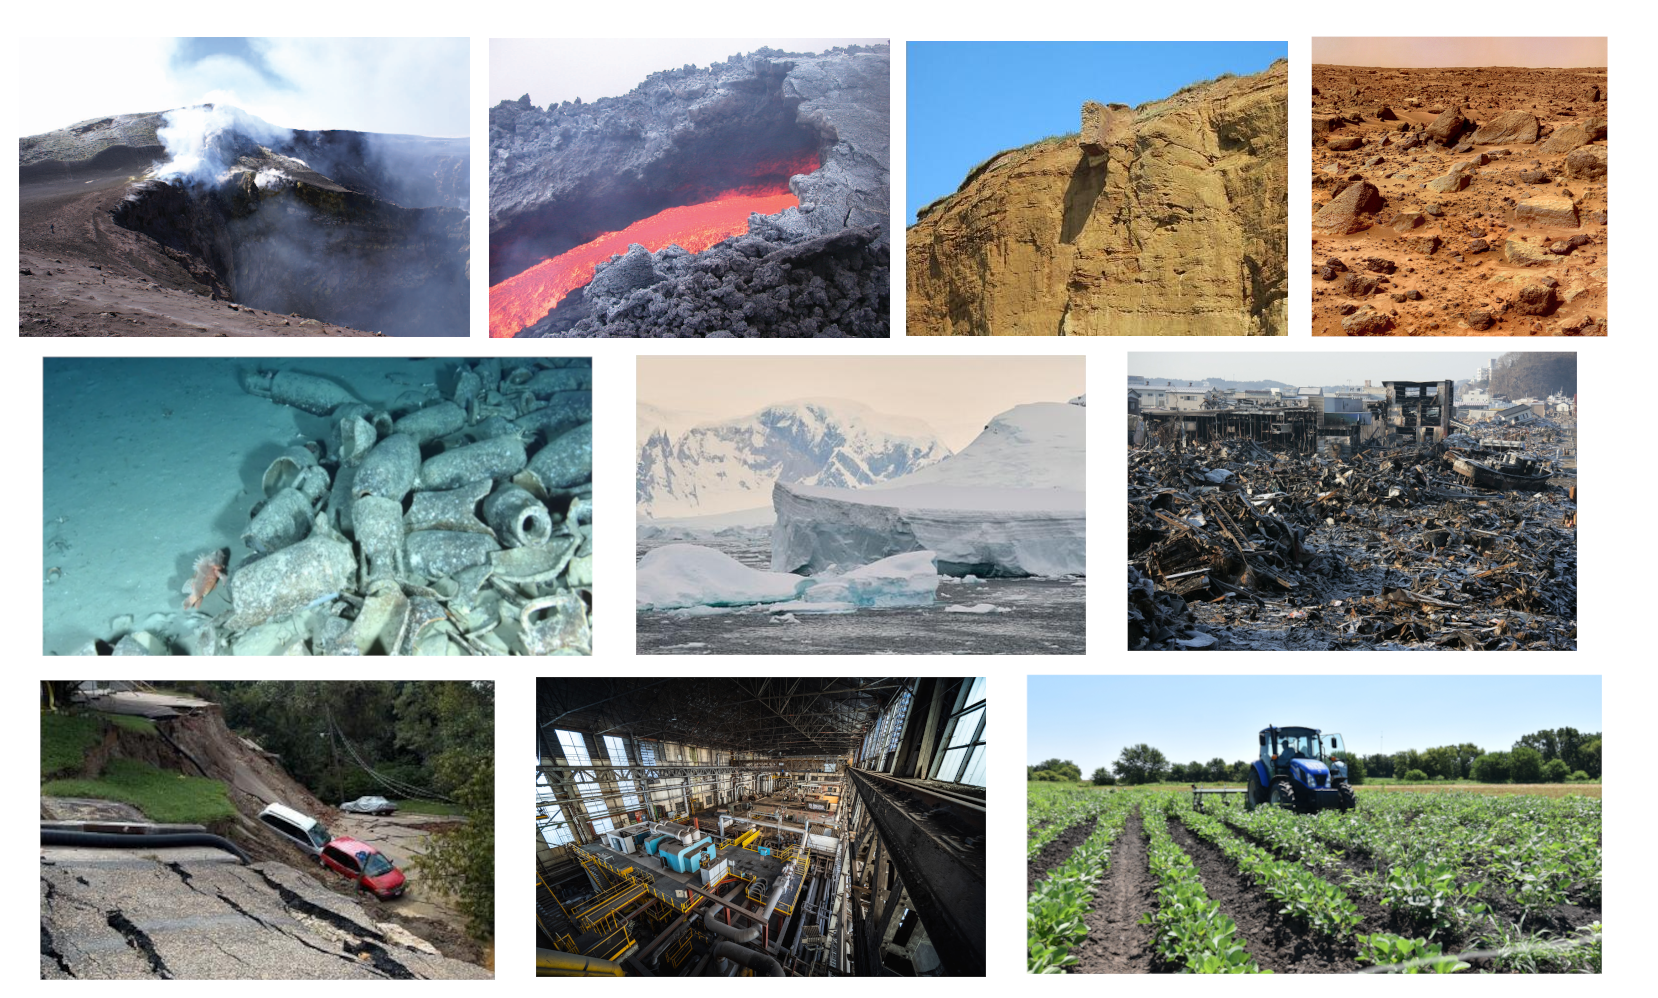
\includegraphics[width=0.85\textwidth]{Images/img_ch1/ExtremeUNstructured.png}
    \caption[Examples of unstructured and extreme environment]{Unstructured and extreme environment, in order from left to right and top to down: Mount Etna, Etna eruption, cliff, Mars, underwater archaeological site, Antarctica, Kasenumma city after the Great East Japan Earthquake, landslide,  power plant, farm field.}
    \label{fig:extreme_unstructured}
\end{figure}
Figure \ref{fig:extreme_unstructured} represents some examples of the domain of interest, referred to as \textbf{unstructured environments}. In particular, locations such as volcanoes, space, deep ocean, and disaster sites are referred to as \textbf{extreme environments}, and here more than in other places, the usage of autonomous systems is fundamental to complete different tasks\cite{Vulcanic_Survey}\cite{UnstructuredHOW}\cite{SearchandRescue}.

Extreme environments contain many rough 
terrains that limit the movement of robots, such as steep slopes, cliffs, and rubble areas, and depending on the robot's movement method, 
it may be impossible to reach the destination, or it may take a great deal of time and energy to reach the destination.
Therefore, designing robots for these critical areas is a complex task, involving not only material and electronics durability under extreme conditions, but also advanced 3D perception, environmental awareness, and adaptive locomotion strategies for efficient traversability\cite{TerrainTraversability}\cite{FieldRobots}.

This research focuses on environments composed of flat land and uneven terrain, as well as steeply sloping terrain made of rocks.
In the next section, the state-of-the-art robotics hardware is presented, to highlight the limitations of the classical approach, and introduce novel solutions, similar to the one discussed here. 

\section{Field Robots, different locomotions}
\label{sec:field_robots}
Autonomous and remotely operated machines working in unstructured environments are part of the \textbf{field robotics} research\cite{FieldRobots}. Here different cutting-edge systems are summarized and classified based on the type of locomotion solution.  


\subsection{Wheeled Robots}
\label{subsec:wheeled_robots}

Locomotion on wheels is the most common human transportation system, and the majority mobile robots are also based on this solution. Moving on wheels ensures high speed at low effort, and traversability can be improved with state-of-the-art suspension systems and mechanical structures. 

These types of robots are typically designed for flat terrains, with some robustness against possible roughness. Now some cutting-edge examples are presented.  

ECHO (see Fig.\ref{fig:ECHO}) is a four-wheeled robot to study emperor penguins' behavior, able to move in the Antarctic\cite{WHOI_ECHO} continent. Another example is
ROBOVOLC\cite{ROBOVOLC}\cite{Vulcanic_Survey}, represented in Fig.\ref{fig:ROBOVOLC}, is a robotic system moving on wheels even in rocky terrains, designed to help scientists in the exploration of volcanoes. 
As a final example, The 4-wheeled rover EX1 (in Fig.\ref{fig:EX1}) ensures smooth and stable driving at increased speed over loose soils, irregular hard surfaces, and hazard-abundant landscapes, thanks to its mechanically hybrid suspension system\cite{EX1}. 

\begin{figure}[H]
    \centering
    \subfloat[ROBOVOLC in mount Etna.\label{fig:ROBOVOLC}]{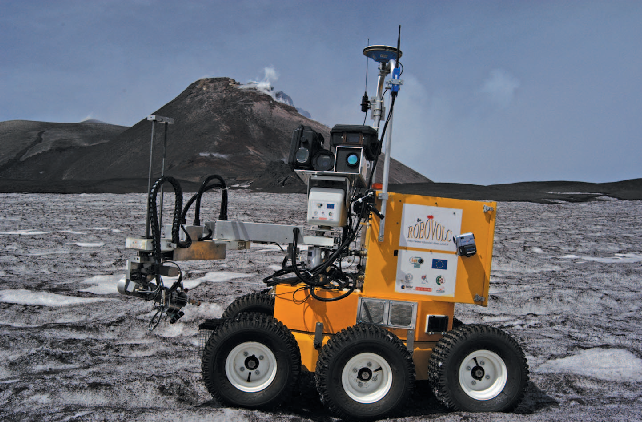
\includegraphics[width=0.28\textwidth]{Images/img_ch1/ROBOVOLC.png}}
    \subfloat[ECHO in Antartica.\label{fig:ECHO}]{
    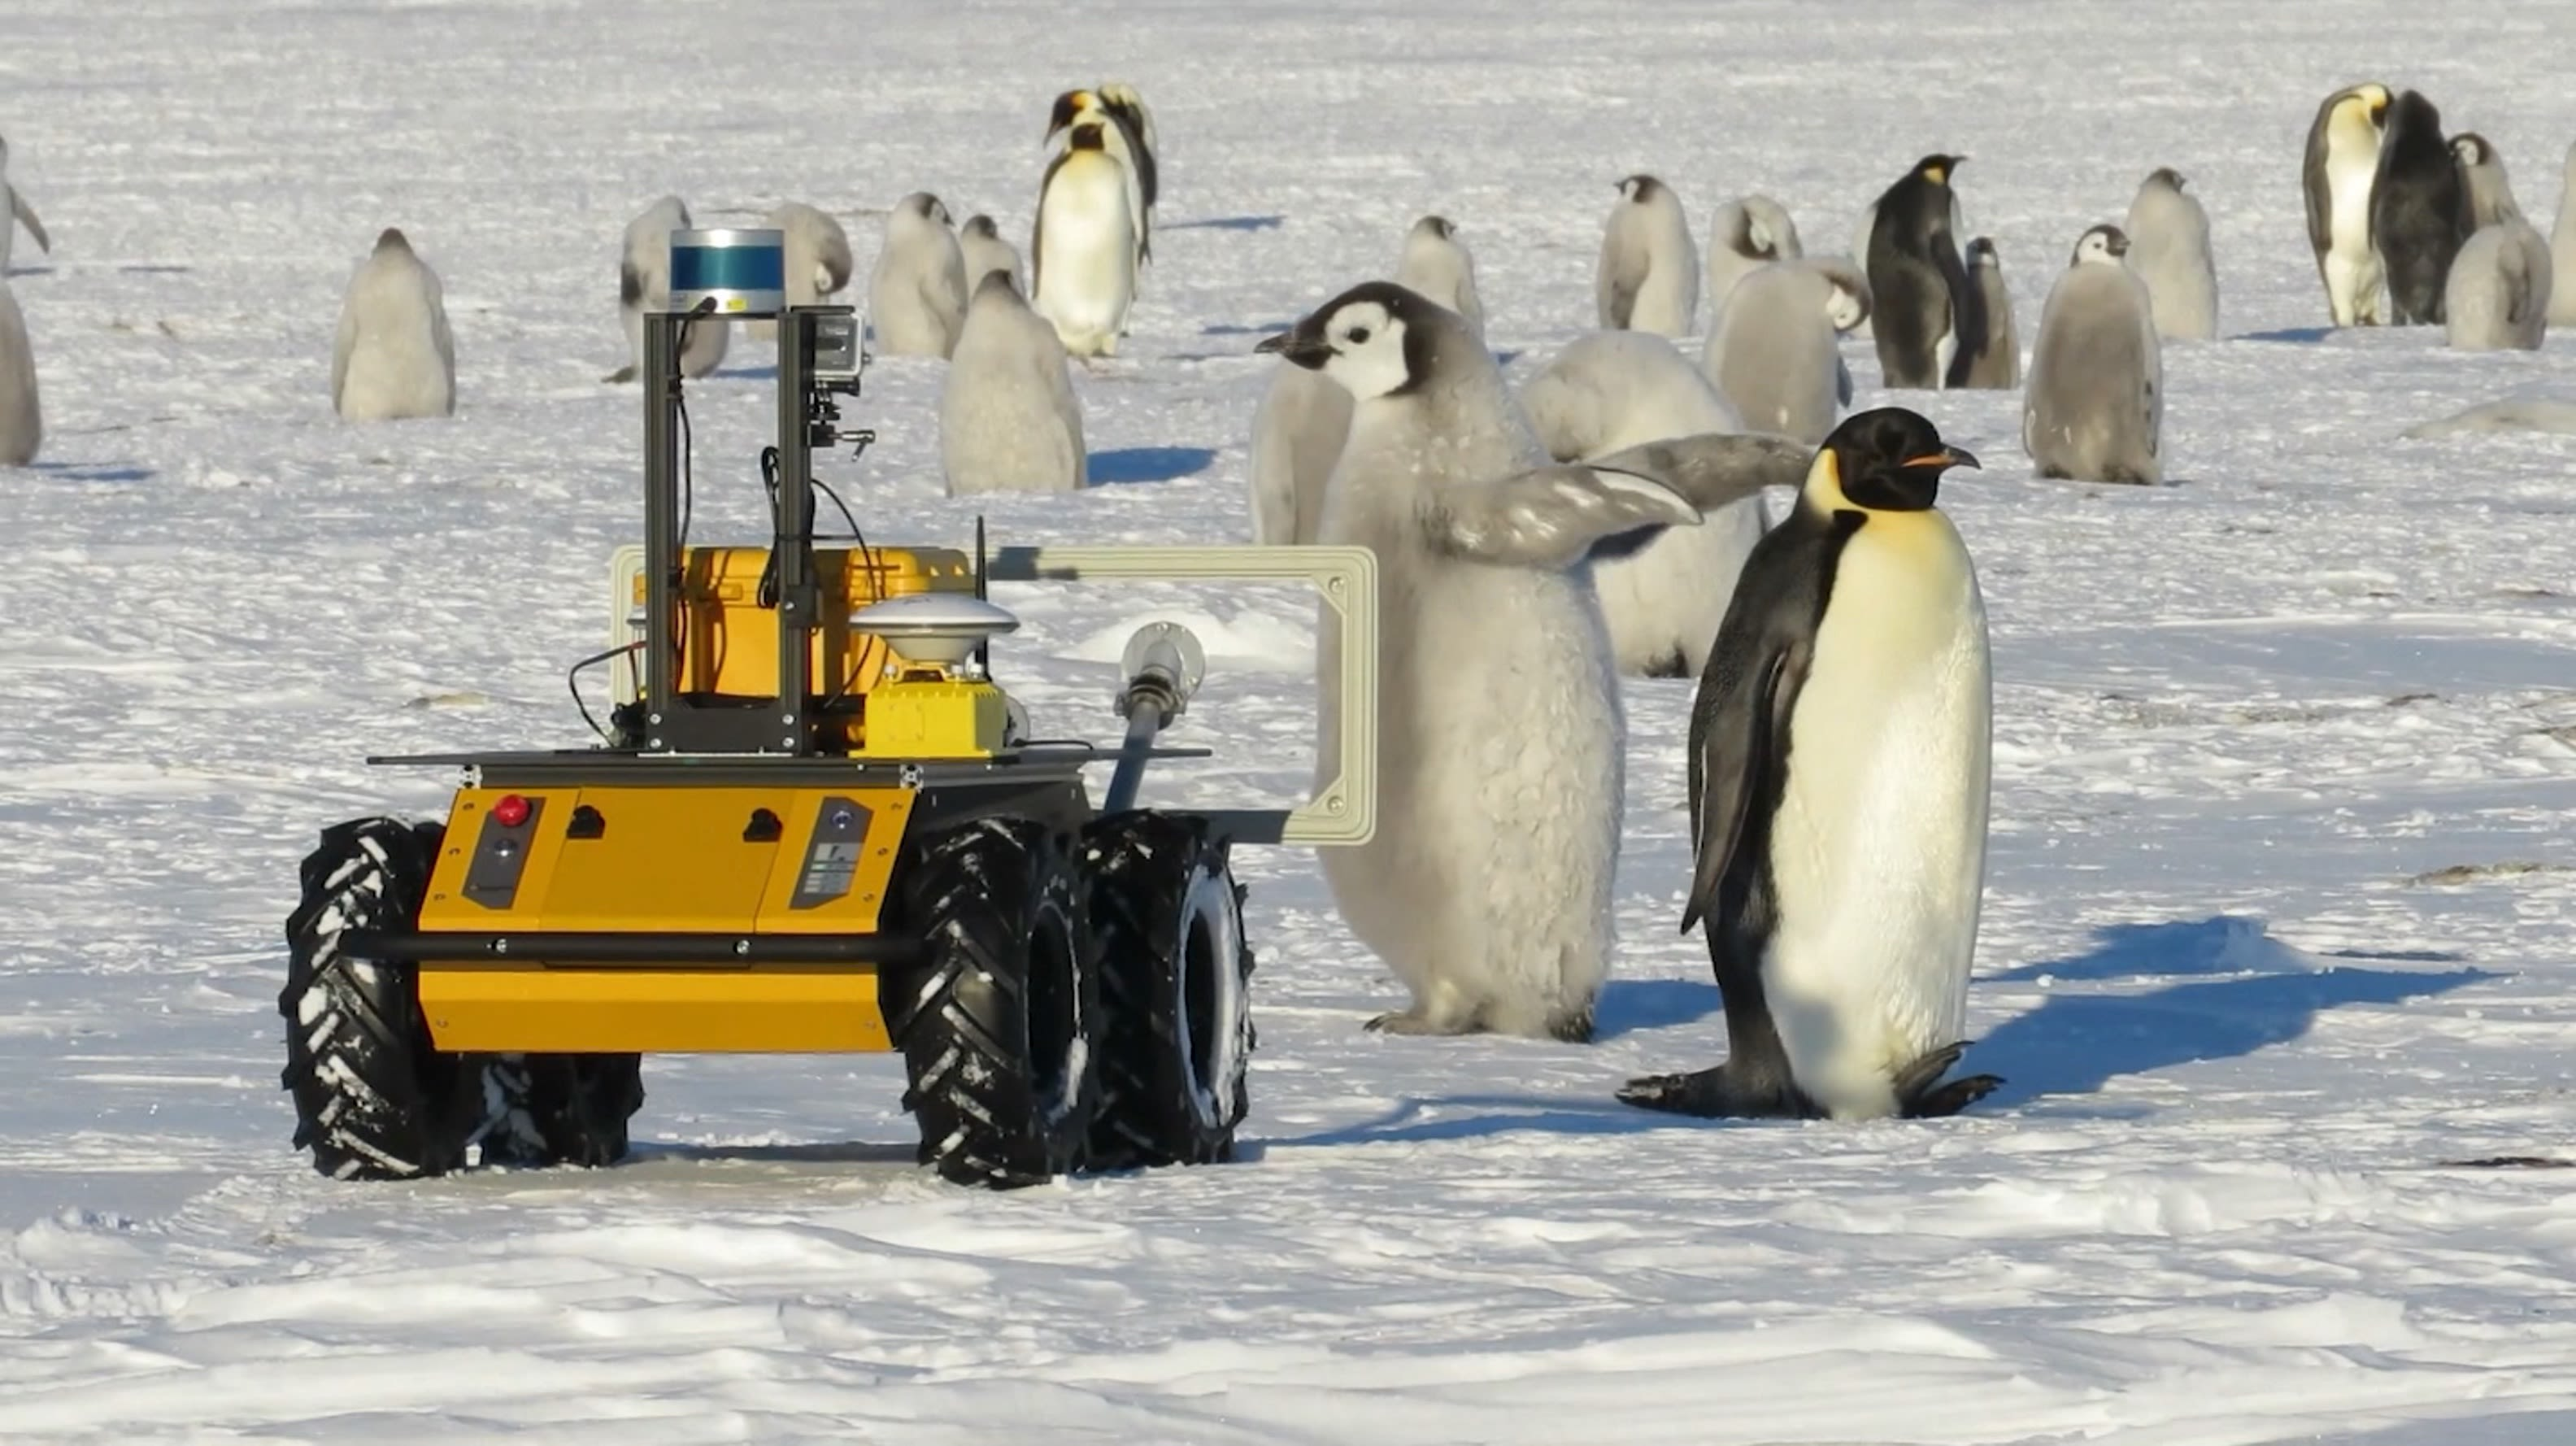
\includegraphics[width=0.32\textwidth]{Images/img_ch1/ECHO_antartica.jpg}}
    \subfloat[EX1 high-speed rover.\label{fig:EX1}]{
    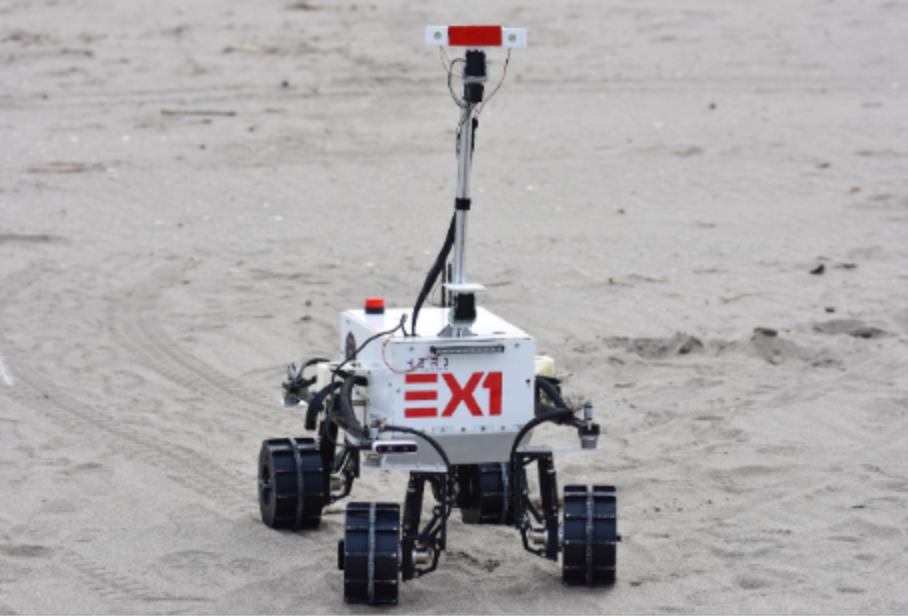
\includegraphics[width=0.28\textwidth]{Images/img_ch1/EX1.png}}
    \caption[Wheeled robot]{Wheeled robots}
    \label{fig:wheeled}
\end{figure}
The robots described here are different from other classical simple and rigid wheeled structure solutions. However, in muddy or very rough terrain, tracked locomotion is the most suitable.

\subsection{Tracked Robots}
\label{subsec:tracked_robots}

For their larger contact area with the ground,
tracked robots are used when high traction and payload capacity are required. 
Examples, represented in Fig.\ref{fig:tracked} are Quince \cite{Quince}\cite{FukushimaPlant}, a rescue robot developed by Satoshi Tadokor's group, and the tracked vehicles employed during the TRADR\cite{TRADR} project
\cite{Amatrice}\cite{SearchandRescue}. 

\begin{figure}[H]
    \centering
    \subfloat[Quince.\label{fig:WheelFly_robot}]{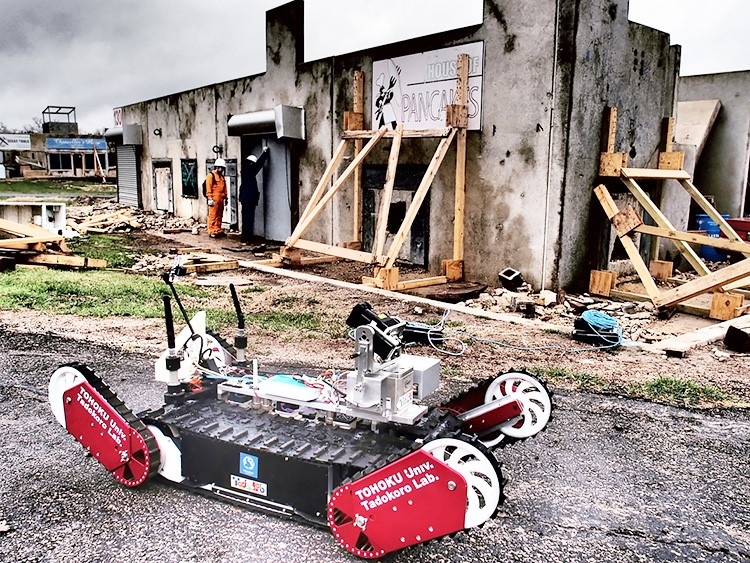
\includegraphics[width=0.4\textwidth]{Images/img_ch1/QuinceRobot.jpg}}
    \subfloat[rover form TRADR project, Amatrice.\label{fig:TRADR}]{
        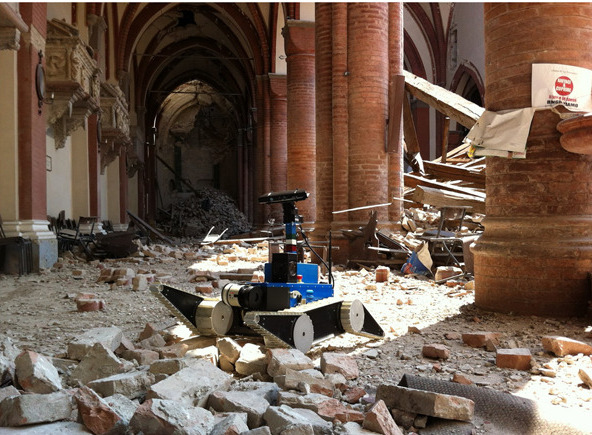
\includegraphics[width=0.4\textwidth]{Images/img_ch1/TRADR_UGV.jpg}}
    \caption[Tracked robots for search and rescue]{Tracked robots for search and rescue activities}
    \label{fig:tracked}
\end{figure}
With tracks, more types of terrains are traversable, at the cost of less energy efficiency than wheeled robots. 
However, there are still traversability limitations due to the required "continuous" trajectory on the ground, intrinsic both for tracked and wheeled locomotion. 


\subsection{Legged Robots}
\label{subsec:walking_robots}

The discrete ground interaction of legged robots solves
the problem mentioned above. This locomotion has been inspired by what Mother Nature has created over hundreds of millions of years of evolution and refinements\cite{Todd}.   

HyQ\cite{HyQ_website}\cite{HyQpaper} is a quadruped from the Italian Institute of Technology (IIT), ANYmal (in Fig.\ref{fig:ANYmal_outdoor} and \ref{fig:ANYmal_fire}), developed by ANYbotics for autonomous industrial inspection, and now enabling some of the most advanced legged locomotion capabilities 
\cite{LeggedRealWorld}\cite{AnymalDocThesis}\cite{LeggedRealWorld}\cite{SearchandRescue}.
Finally, from the researches on legged locmotion by Mark Raibert\cite{Raibert}, Boston Dynamics' Spot\cite{spot_website}  (in Fig.\ref{fig:Spot}) was one of the first machines to spark market interest in legged robots.
\begin{figure}[H]
    \centering
    \subfloat[ANYmal outdoor.\label{fig:ANYmal_outdoor}]{
        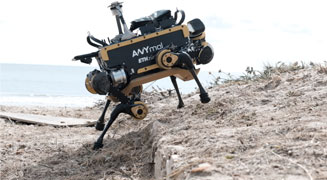
\includegraphics[width=0.3\textwidth]{Images/img_ch1/anymalOutdoor.png}
    }
    \subfloat[ANYmal during a fire.\label{fig:ANYmal_fire}]{
        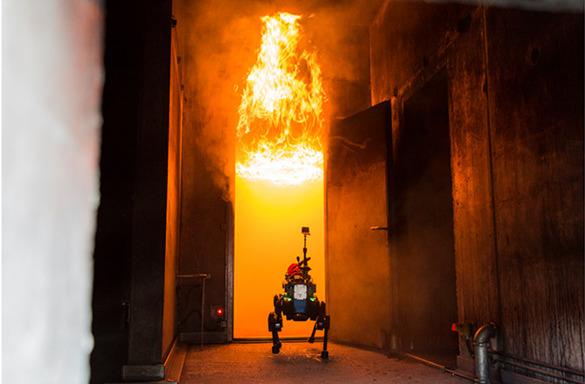
\includegraphics[width=0.3\textwidth]{Images/img_ch1/ANYmal_fire.jpg}
    }
    \subfloat[Boston Dynamics Spot.\label{fig:Spot}]{
        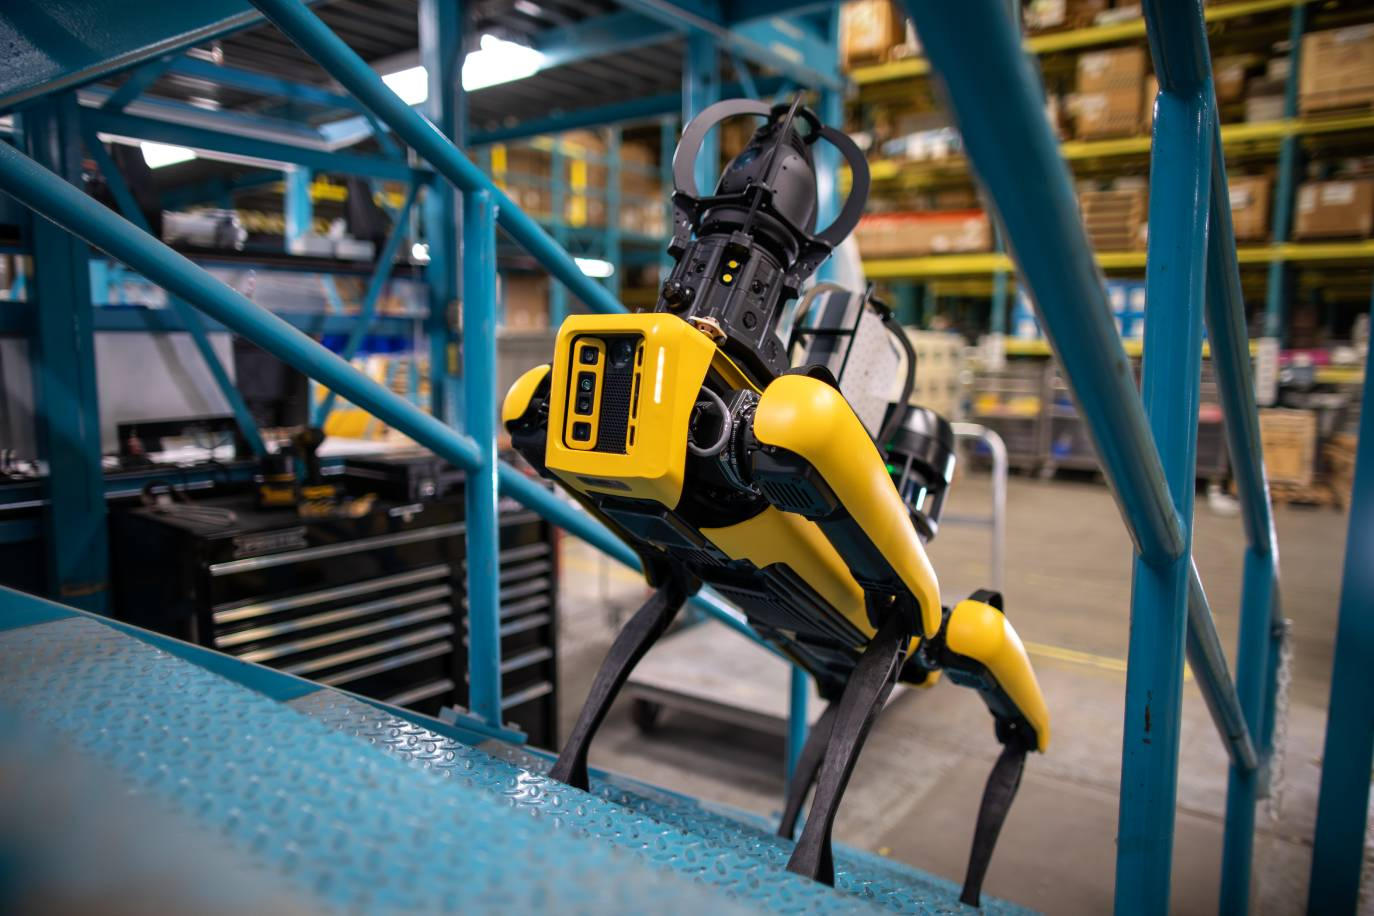
\includegraphics[width=0.3\textwidth]{Images/img_ch1/Spot.jpg}
    }
    \caption[Quadruped legged robots]{Examples of quadruped legged robots in unstructured environment.}
    \label{fig:WalkingRobots}
\end{figure}
The higher terrain adaptability again comes with costs in terms of energy efficiency and much more complexity in the development and design of those systems. 

Bipedal, hexapod, and even octopod legged robots exist, and it is relevant to highlight the increase of payload and stability when using more legs, and the manipulation ability with two upper arms in humanoids\cite{HumanoidRobot}.

The concept of legged locomotion can be extended into limbed robots, which use their "limbs" to move the base and manipulate the environment, without having to differentiate arms and legs as humanoid does.  

\subsection{Multilimb Robots}
\label{subsec:multilimb_robots}

Multilimbed robots are a wide class of robots\cite{Koyachi}, and legged machines are a subclass of this. 
Classical walking machines use simple foot tips and specific leg structures to interact with the environment and generate the necessary reaction forces to achieve motion. Multilimbed machines instead can employ different types of end effectors attached at the limb-end, depending on the task, such as magnetic modules \cite{MAGNEKO}, vacuum suction units\cite{suctionfoottip}, and passives spine grippers\cite{passiveSpineTohoku}, to list a few possibilities.
Furthermore, the limbs are properly structured to enhance the workspace, and sometimes redundant designs are employed. 

Particular types of multilimbed machines are climbing robots, designed to move on high slopes, vertical surfaces, or even on the ceiling. An example is the JPL/NASA LEMUR3 robot\cite{LEMUR3} (see Fig.\ref{fig:LEMUR3}), enabling access to previously inaccessible but scientifically relevant areas for space missions. In general, climbing robots lose performance when walking on the ground because designed for optimized climbing locomotion,  
SCALER\cite{SCALER} instead, guarantees fast locomotion also on the ground, and a new gait using the reconfigurable base, as represented in Fig.\ref{fig:SCALER}
\begin{figure}[H]
    \centering
    \subfloat[LEMUR3.\label{fig:LEMUR3}]{
    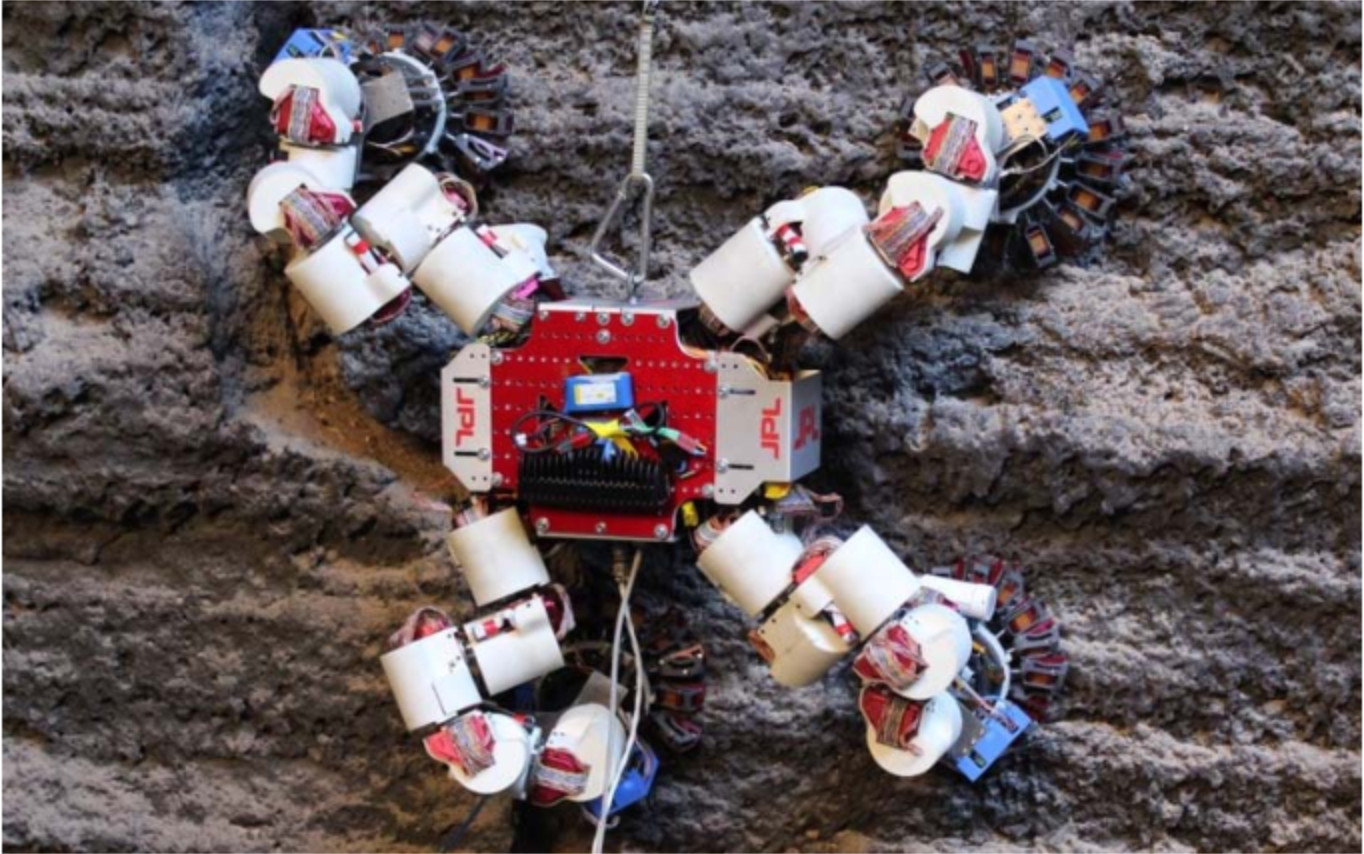
\includegraphics[width=0.55\textwidth]{Images/img_ch1/LEMUR3.png}}
    \subfloat[SCALER.\label{fig:SCALER}]{
    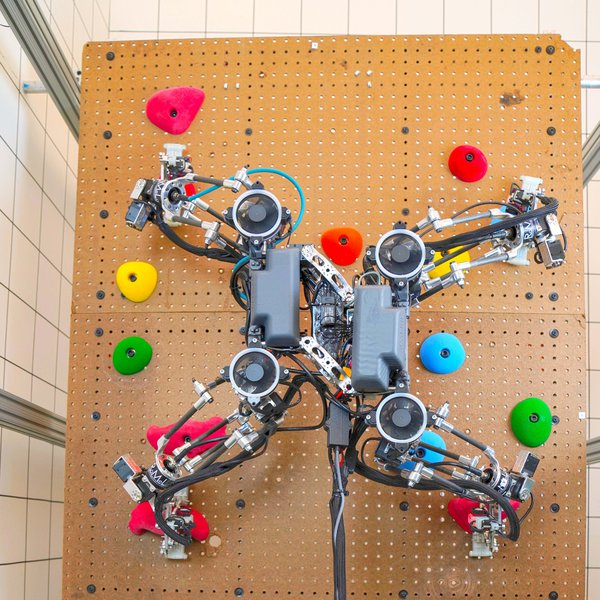
\includegraphics[width=0.35\textwidth]{Images/img_ch1/SCALER.jpg}}  
    \caption[Multi-Limb climbing robots]{Multi-limb climbing robots.}
    \label{fig:Climbing}
\end{figure}
An example of a multifunctional multilimbed robot is SCAR-E, an omnidirectional hexapod designed by the team of the Asteroid Mining Corporation (AMC). This robot structure enables horizontal and vertical locomotion in uneven environments, and multiple task execution with an interchangeable end effector\cite{SCARE_gripper}\cite{SCAR-E}. Figure \ref{fig:SCARE} represents the robot with simple feet and the designed soft gripper for its mission. Furthermore, the increased workspace of the limb allows it to reach tools carried on the base, and change the end effector depending on the task.

\begin{figure}[H]
    \centering
    \subfloat[SCAR-E Concept.\label{fig:SCARE_Concept}]{
        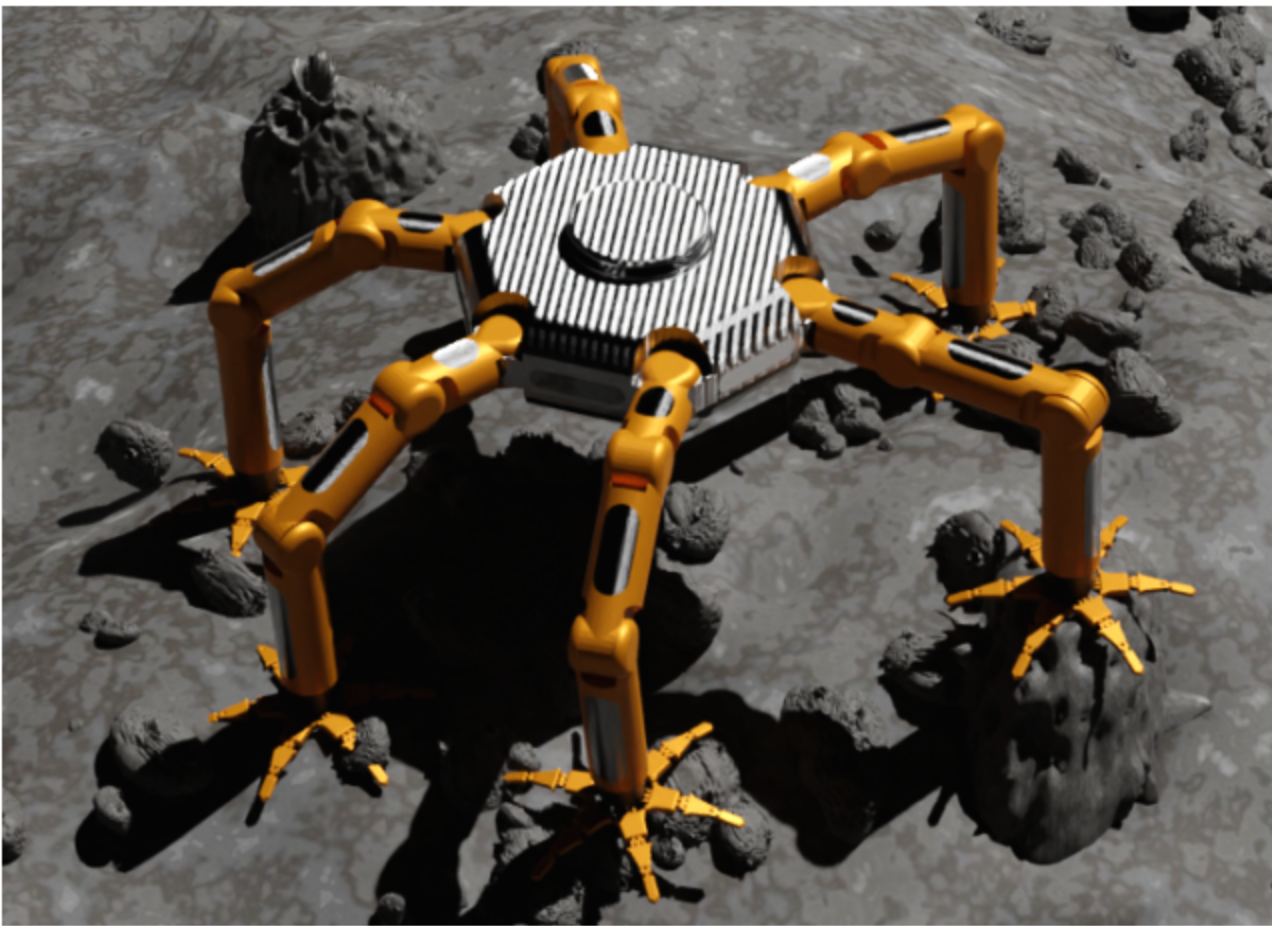
\includegraphics[scale=0.13]{Images/img_ch1/SCAR-E_concept.png}
    }
    \subfloat[SCAR-E Multi-limb Robot.\label{fig:SCARE_Robot}]{
        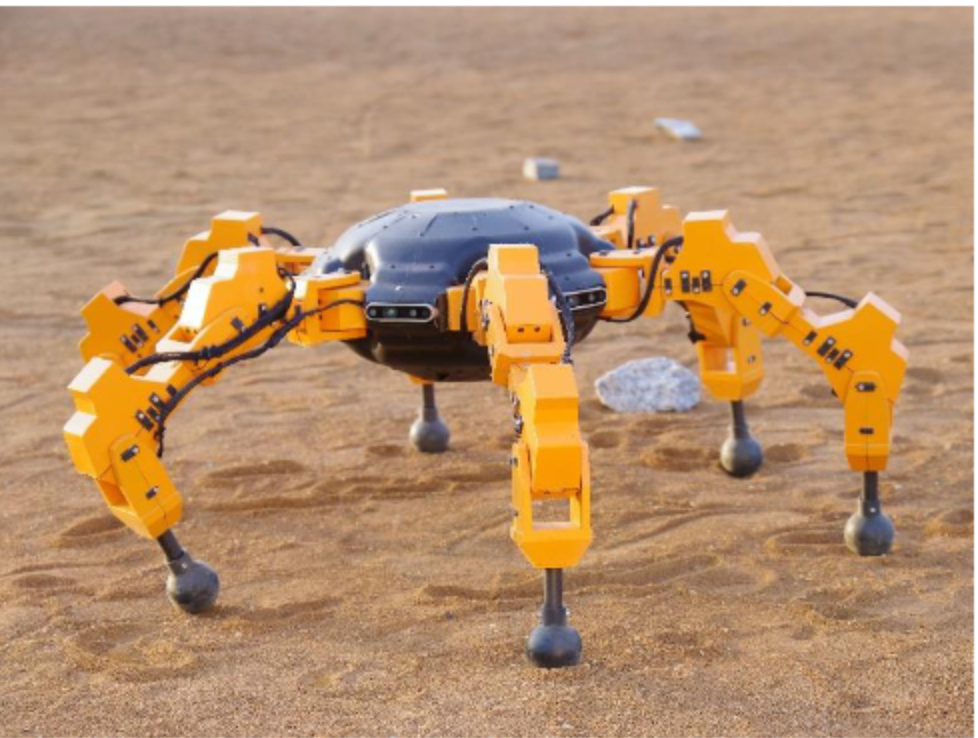
\includegraphics[scale=0.18]{Images/img_ch1/SCAR-E.png}
    }
    \subfloat[Soft gripping system.\label{fig:SCARE_Gripper}]{
        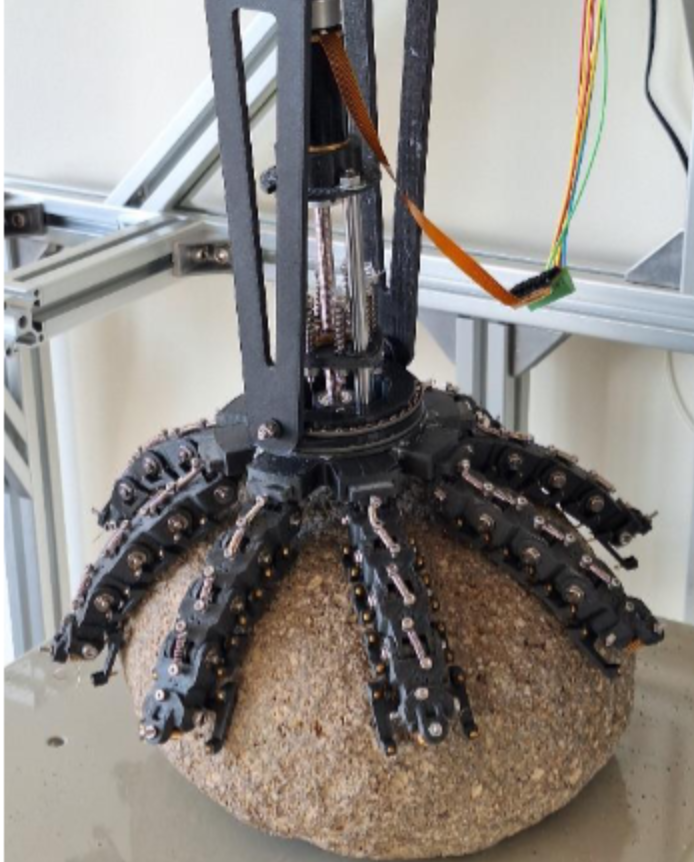
\includegraphics[scale=0.15]{Images/img_ch1/SCAR-E_Gripper.png}
    }
    \caption[Asteroid Mining Corporation (AMC) SCAR-E.]{AMC SCAR-E multi-limb robot for asteroid mining\cite{SCARE_gripper}\cite{SCAR-E}.}
    \label{fig:SCARE}
\end{figure}


Other locomotion solutions exist for other domains, such as propellers and thrusters for air and underwater navigation, enabling flying and swimming locomotion.
The problem with flying systems is that in general narrow navigation is complex, the cost of hovering is non-negligible, and payload capabilities are limited. 

Table \ref{table:locomotion_summary} summarizes the performance of the different classical locomotion forms as an average of traversability and energy efficiency.

\begin{table}[H]
\centering 
    \caption{Summary of locomotion performances for different terrains and tasks, where the average performance is measured from 0 to 3}
    \label{table:locomotion_summary}
    \begin{tabular}{ c }
    \textbf{Limb Joints Motors}
    \end{tabular}
    \begin{tabular}{| c | c | c | c | c | c |}
    \hline
    \rowcolor{bluepoli!40}
%    \rowcolor{bluepoli!40}
     \textbf{Task} &  Wheeled & Tracked & Walking & Climbing & Flying\T\B \\
    \hline \hline
    \textbf{Flat Terrains} & \cellcolor{bluepoli!20}3 & 2 & 1 & 0  & 2  \T\B\\
    \hline 
    \textbf{Rough Terrains} & 0 & 2 & \cellcolor{bluepoli!20}3 & 1  & 2 \T\B\\
    \hline
    \textbf{Rocky Slopes} & 0 & 1 & 1 & \cellcolor{bluepoli!20}3 & 2 \T\B\\
    \hline
    \textbf{Vertical Walls} & 0 & 0 & 0 & \cellcolor{bluepoli!20}3 & 2 \T\B\\
    \hline
    \textbf{Manipulation} & 0 & 0 & 0 & \cellcolor{bluepoli!20}3 & 0 \B\\
    \hline
    \end{tabular}
\end{table}


In conclusion, for the complex terrain considered in this research, which includes sloping rocky surfaces, flat ground, and uneven terrain, none of the proposed solutions achieve the optimal balance between energy efficiency and mobility.
To solve the issue of adaptability to different terrain conditions, without sacrificing efficiency or speed, hybrid forms of locomotion and multimodal robot designs exist. 

\subsection{Hybrid and Multimodal Robots}
\label{subsec:hybrid_robots}

The combination of multiple forms of locomotion is an active research topic, from the cooperation of more robots
\cite{MultimodalityROBOTS}, to the possibility of integrating multiple functionalities on a single machine.

Focusing on single-agent systems, 
In literature, the terms hybrid and multimodal are often used interchangeably, here the following differentiation is considered:\\ 
\textit{The locomotion is considered \textbf{hybrid} when a non-conventional solution enables multiple interactions with the environment, based on the same mechanism. \textbf{Multimodality}, on the other hand, involves different forms of movement from multiple integrated actuators, or a reconfiguration of the system structure.}

First, some examples from the hybrid locomotion domain are presented. 

The hybrid form of ANYmal\cite{AnymalDocThesis}\cite{legged-wheeled} (in Fig.\ref{fig:ANYmal_Wheels}) uses non-steerable wheels attached to its legs, allowing the robot to be efficient
on flat as well as agile on challenging terrain. Furthermore, it exploits skating motions with passive wheels, 
reducing the cost of transport
from legged systems. MAMMOTH\cite{MAMMOTH}\cite{MAMMOTH_structure} (in Fig.\ref{fig:MAMMOTH}) is an actively articulated wheel-on-leg rover, capable of traversing obstacles while driving, by reconfiguring its legs. Another example is Q-Whex\cite{QWhex}, a quasi‐wheeled hexapod robot (represented in Fig.\ref{fig:QWhex}), which uses a unique wheel design to traverse different types of irregular terrains. 


\begin{figure}[H]
    \centering
    \subfloat[ANYmal hybrid locomotion\label{fig:ANYmal_Wheels}]{
        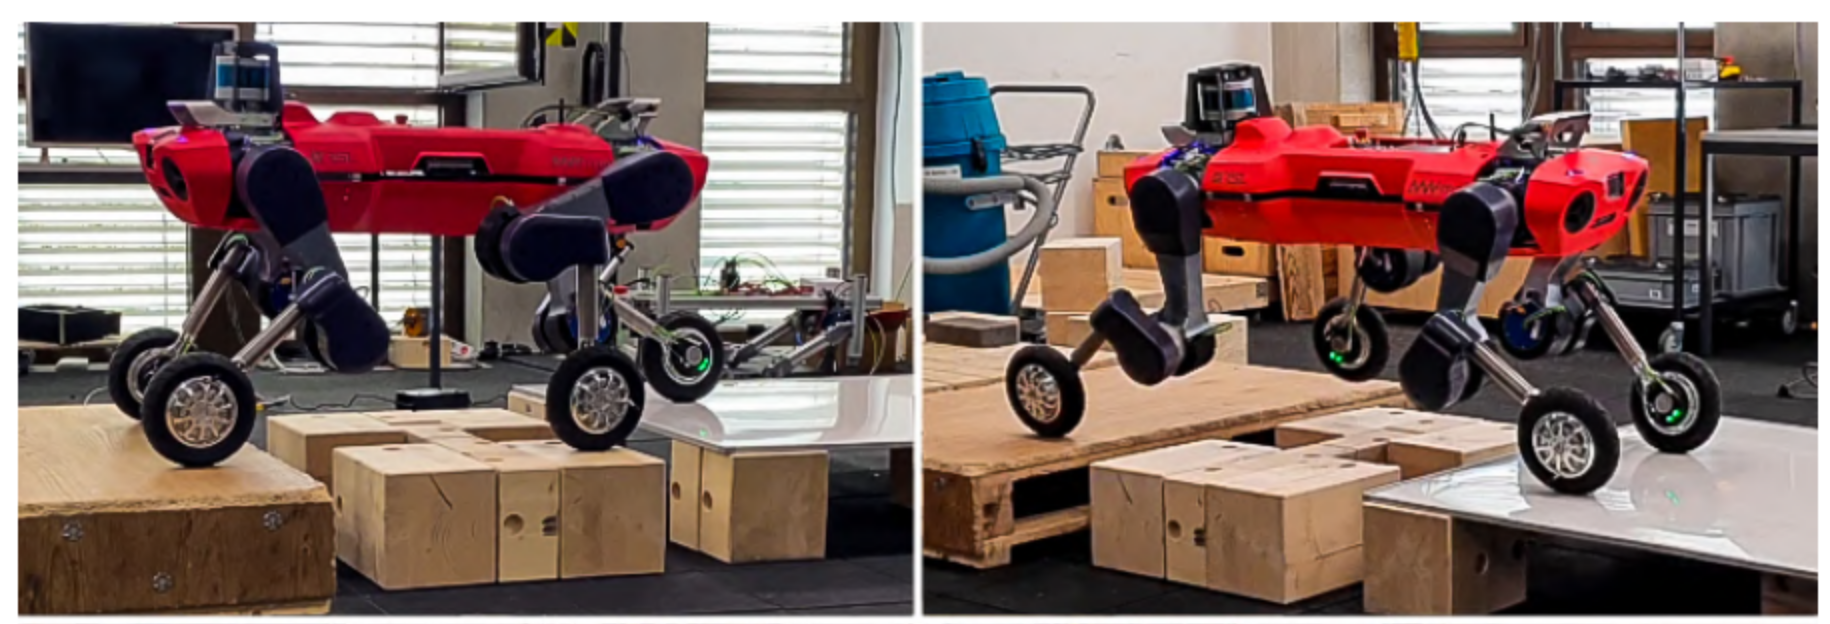
\includegraphics[width=0.50\textwidth]{Images/img_ch1/ANYmal_wheels.png}}
    \subfloat[MAMMOTH\label{fig:MAMMOTH}]{
        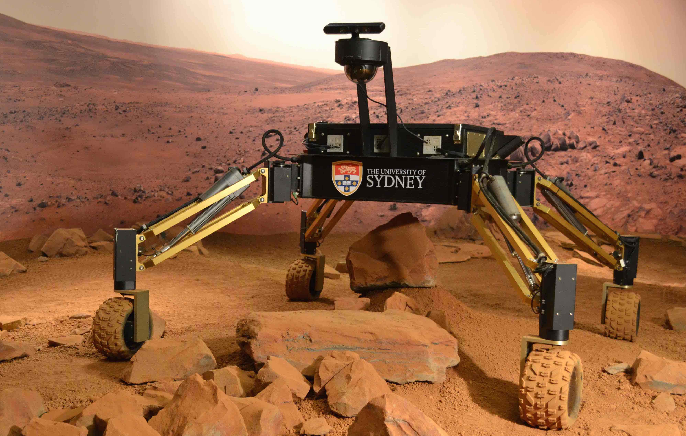
\includegraphics[width=0.25\textwidth]{Images/img_ch1/MAMMOTH.png}}
    \subfloat[Q-Whex \label{fig:QWhex}]{
        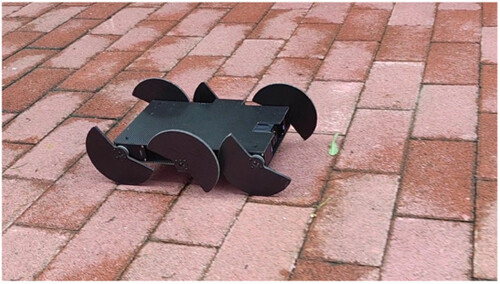
\includegraphics[width=0.25\textwidth]{Images/img_ch1/Q_Whex_quasiWheel.jpg}}
    \caption[Hybrid locomotion examples]{Hybrid locomotion robots examples}
    \label{fig:HybridLeggedWheel}
\end{figure}

The hybrid locomotion solutions described above use particular mechanical structures and adaptability behavior to enhance locomotion, 
when the robot reconfigures its mechanical structure or uses completely different actuators for different motion tasks, it is considered multimodal.

Multi-Modal Mobility Morphobot, or M4\cite{WheelFly} (represented in Fig.\ref{fig:WheelFly}), employs its components in different ways as wheels, thrusters, and legs, and simulates animals' behavior to enable extensive locomotion plasticity.
Examples of robots that remain on the ground are the reconfigurable legged-tracked AZIMUT\cite{LegsTracks_Azimut}
and the prototype legged-wheeled hexapod robot\cite{Hexapod_LegWheeled}, represented in Fig.\ref{fig:LegMultimodal}.
These two robots reconfigure their mechanical structure to change the ground interaction, furthermore, the hexapod prototype has manipulation capabilities thanks to the additional stability derived from using more legs. 

\begin{figure}[H]
    \centering
    \subfloat[Wheel mode.\label{fig:WheelFly_robot}]{
        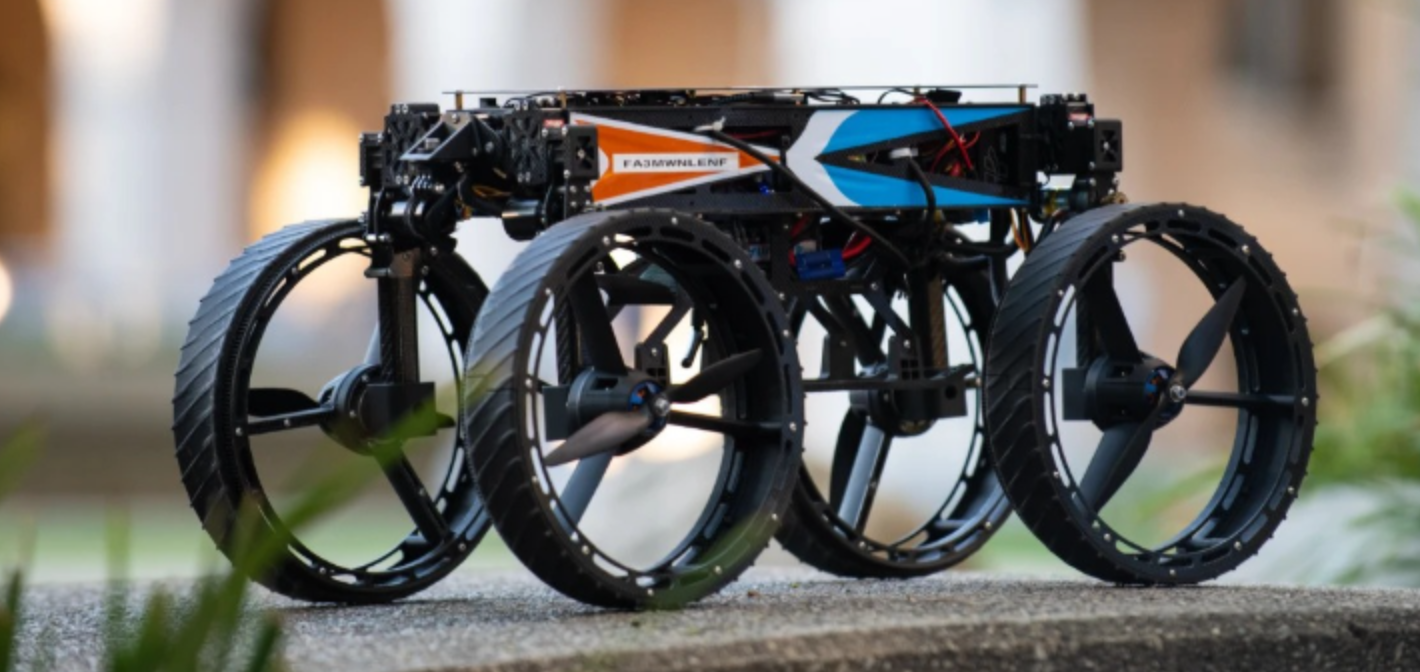
\includegraphics[width=0.4\textwidth]{Images/img_ch1/WheelFly_robot.png}}
    \subfloat[Locomotion transformation seqence.\label{fig:WheelFly_transformation}]{
        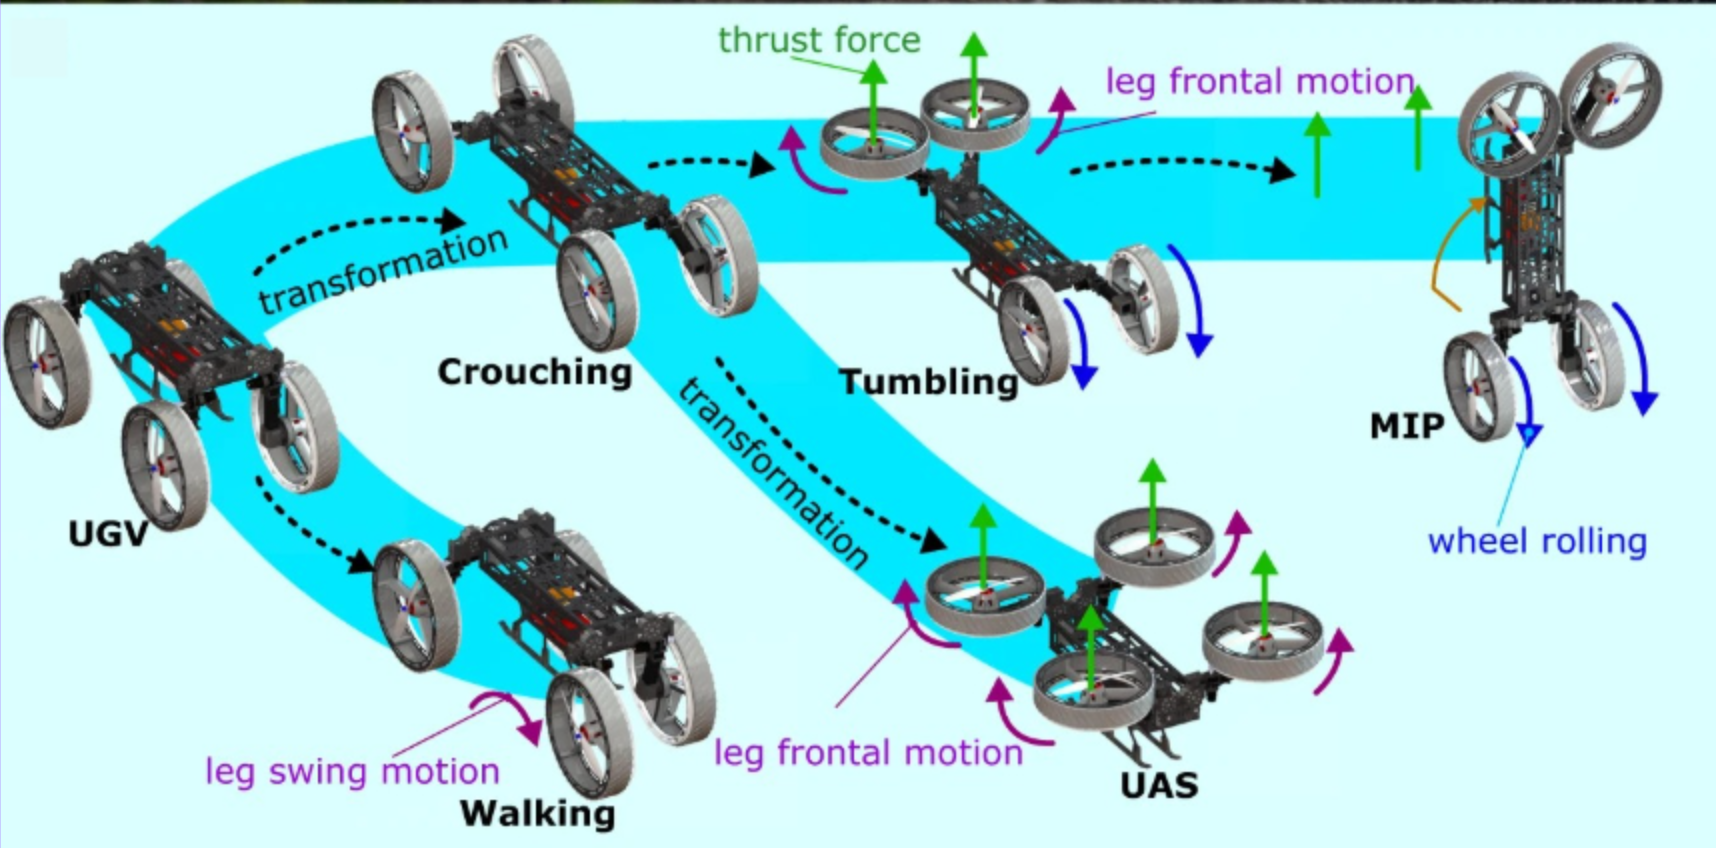
\includegraphics[width=0.55\textwidth]{Images/img_ch1/WheelFly_transformation.png}}
    \caption[Morphobot, driving-flying robot]{Morphobot \cite{WheelFly}, a multimodal driving-flying robot}
    \label{fig:WheelFly}
\end{figure}

\begin{figure}[H]
    \centering
    \subfloat[legged-wheeled hexapod.\label{fig:hexapod_Legwheels}]{
        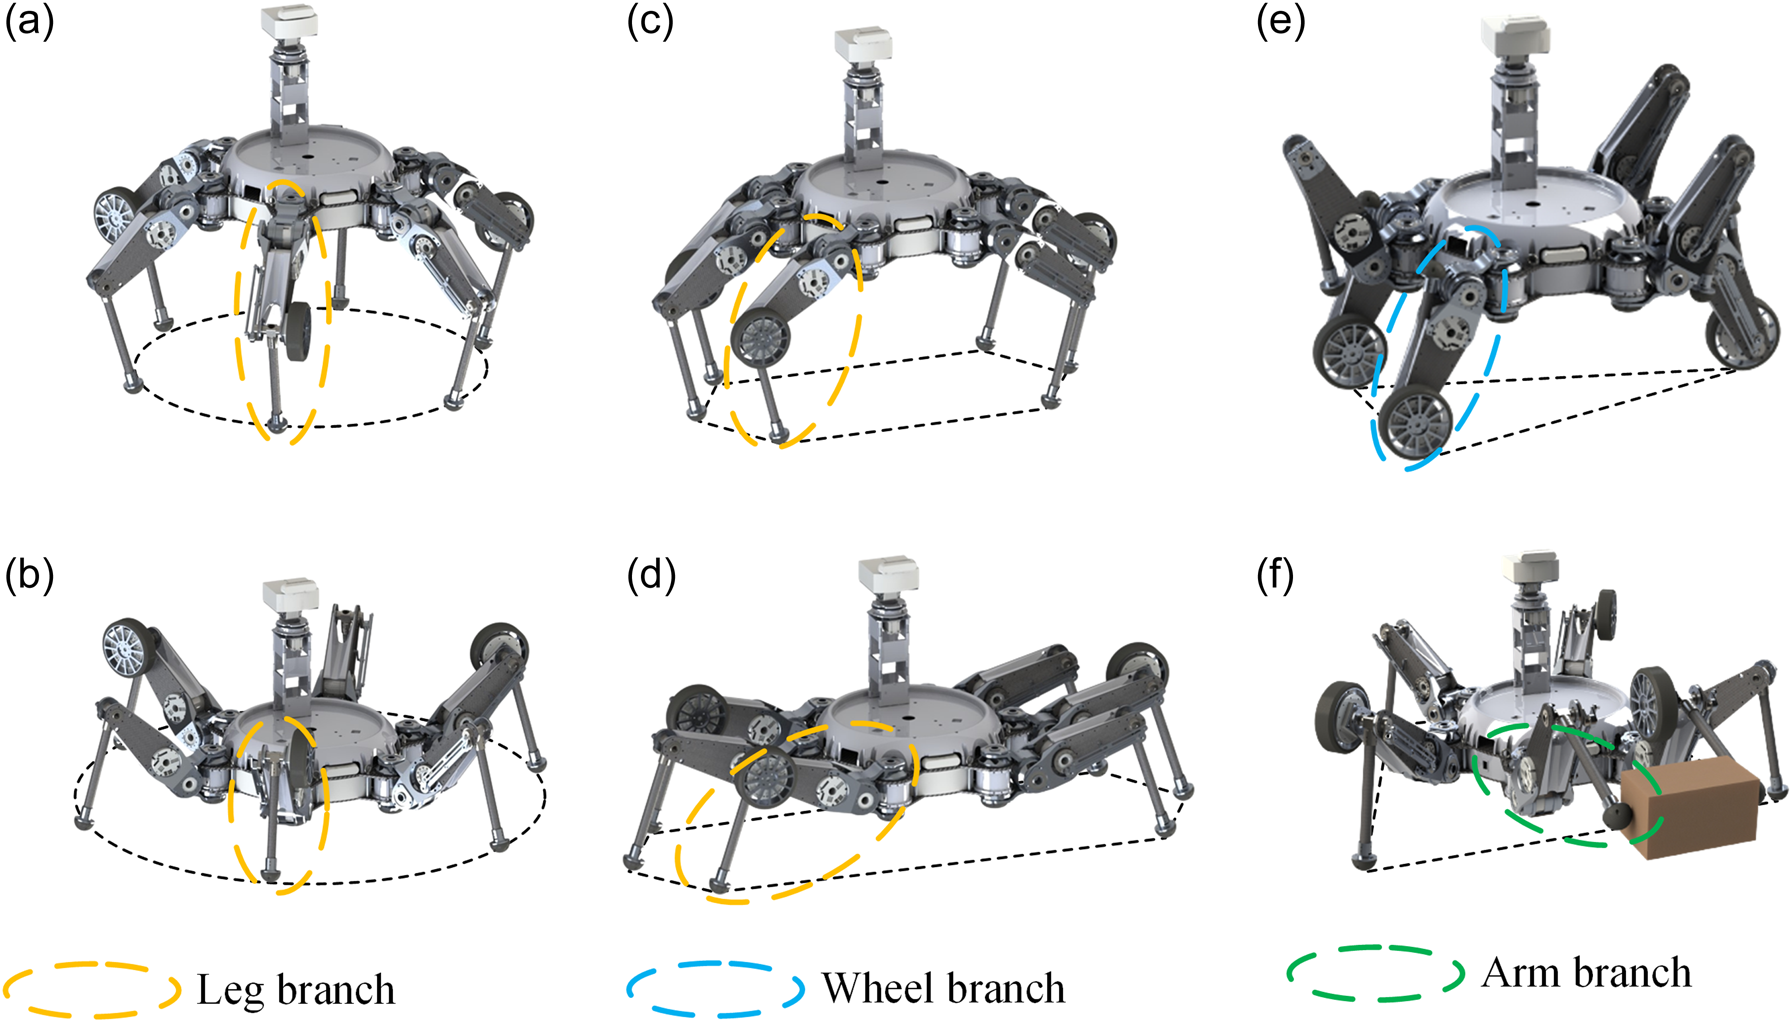
\includegraphics[width=0.6\textwidth]{Images/img_ch1/hexapod_Legweheels.png}}
    \subfloat[legged-tracked AZIMUT.\label{fig:AZIMUT}]{
        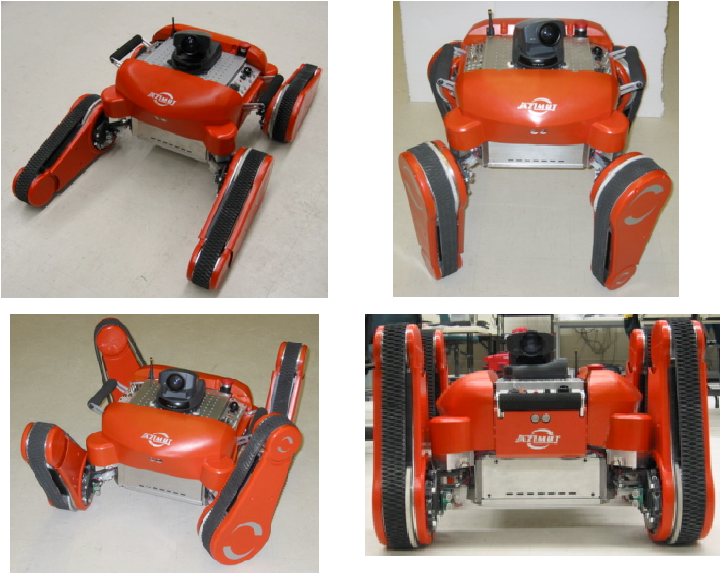
\includegraphics[width=0.4\textwidth]{Images/img_ch1/AZIMUT.png}
    }
    \caption[Multimodal legged robots]{Multimodal robots with different locomotion cpabilities}
    \label{fig:LegMultimodal}
\end{figure}

A cutting-edge robotic system for disaster response is the WAREC-1\cite{WAREC_Site} (and its successor 1R\cite{WAREC1R}), developed from the cooperation of different Japanese research institutes as part of the ImPACT project\cite{JST_IMPACT}. This four-limbed robot has advanced locomotion and manipulation capabilities\cite{WAREC1R_drilling}, transitioning among various locomotion styles, from bipedal/quadrupedal walking, crawling, ladder climbing\cite{WAREC1_book}\cite{WAREC1R}, and even driving with steerable or mecanum wheels.    
Figure \ref{fig:WAREC1} reports the possible manipulation and locomotion capabilities, even in highly unstructured environments with complex tasks to complete and obstacles to traverse. 

\begin{figure}[H]
    \centering
    \subfloat[Manipulation \label{fig:WAREC_manipulation}]{
    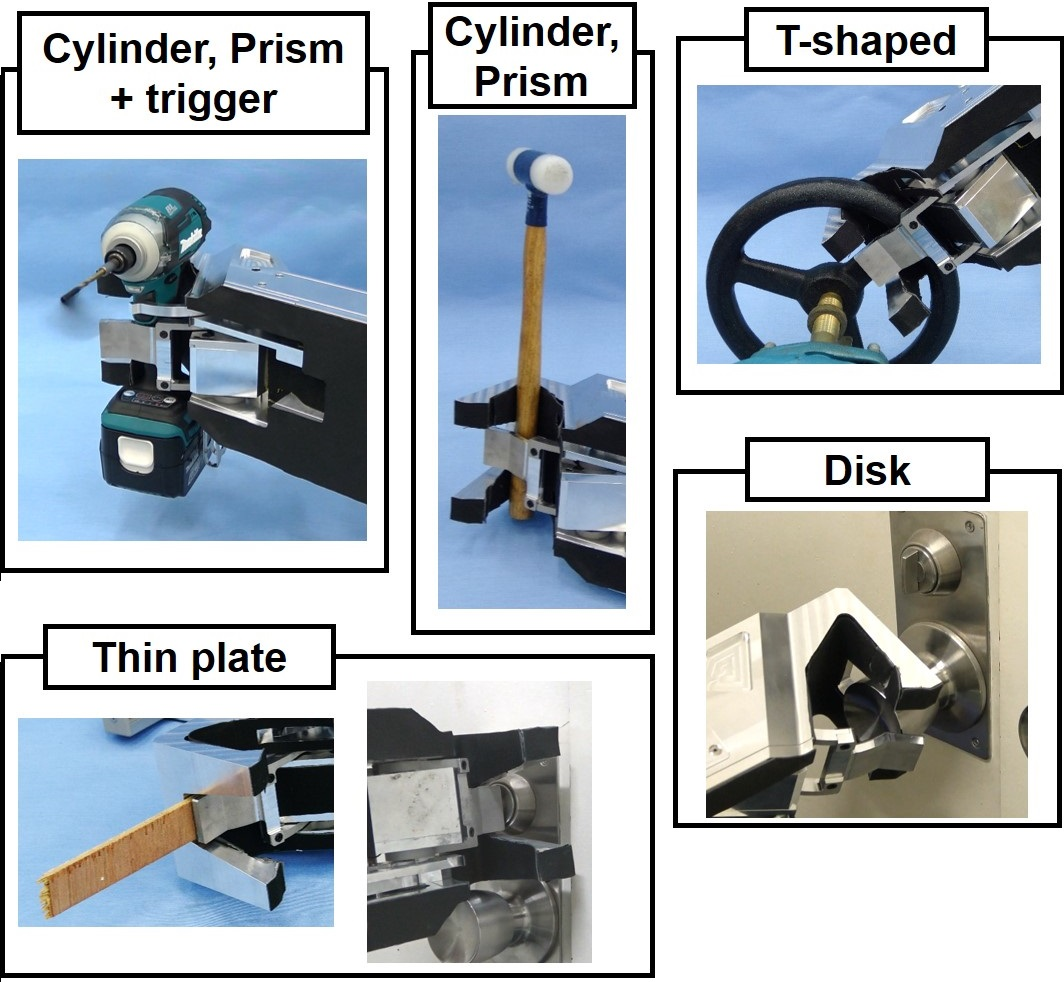
\includegraphics[width=0.3\textwidth]{Images/img_ch1/EE_WAREC1.jpg}}
    \subfloat[Omni wheel end effector\label{fig:WAREC_omniwheel}]{
    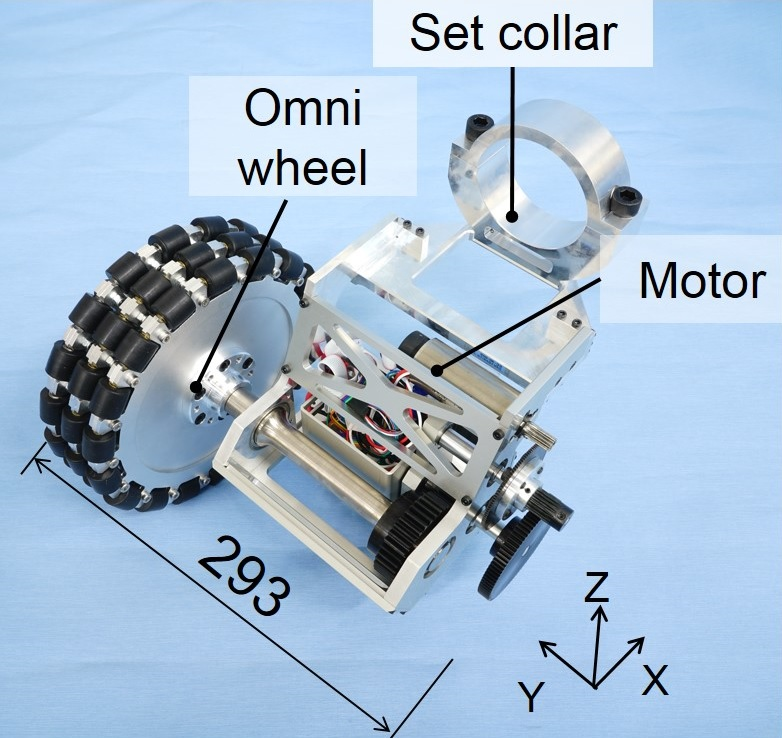
\includegraphics[width=0.3\textwidth]{Images/img_ch1/omniwheel_WAREC1.jpg}}
    \subfloat[Omni wheel driving mode \label{fig:WAREC_driving}]{
    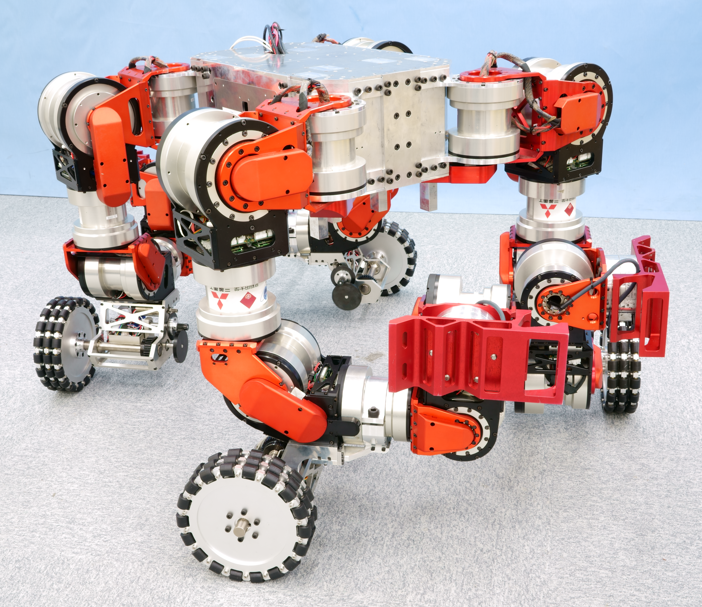
\includegraphics[width=0.3\textwidth]{Images/img_ch1/WAREC1_omniwheel.png}} \\
    \subfloat[WAREC-1R adaptable multimodal locomotion.\label{fig:WAREC_multimodal}]{
    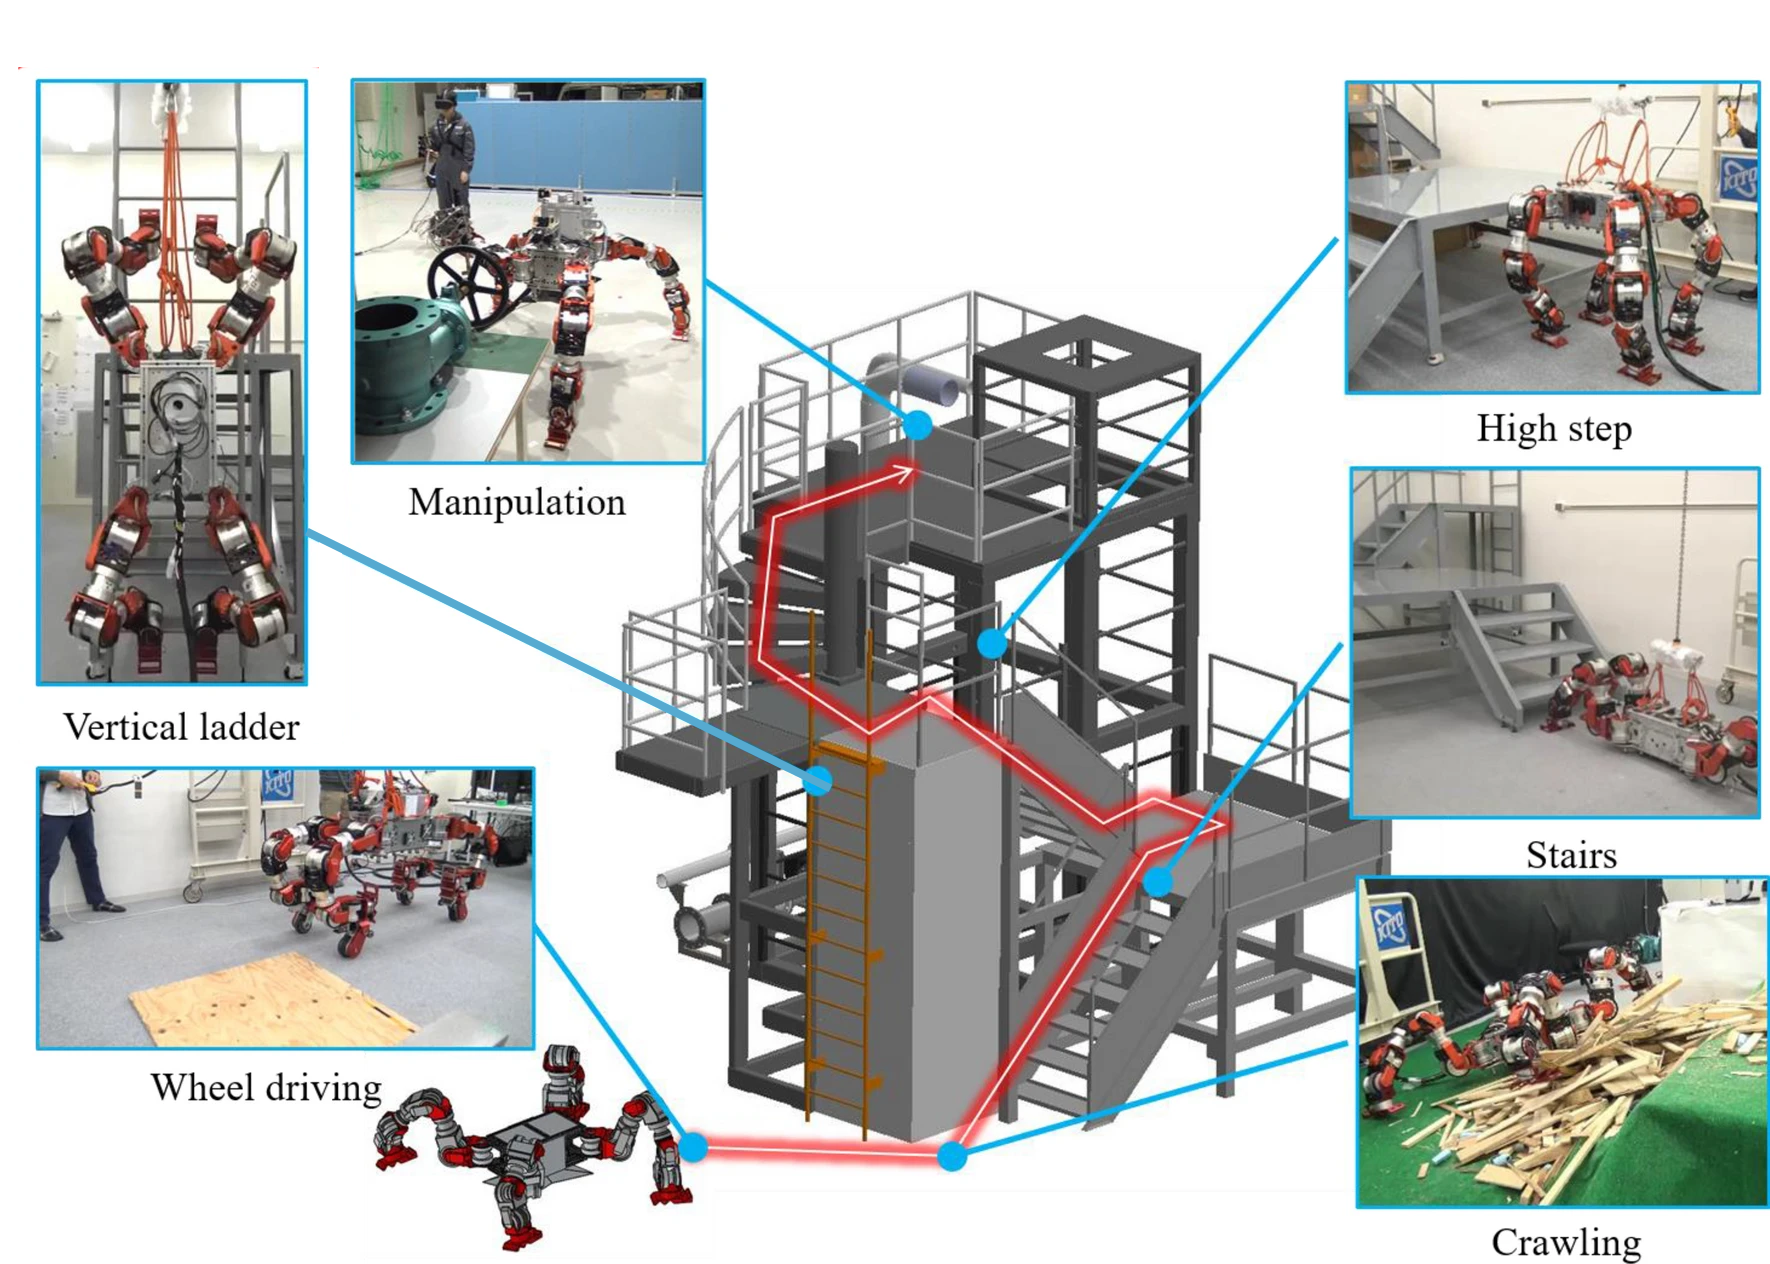
\includegraphics[width=0.9\textwidth]{Images/img_ch1/WAREC1_multimodal.png}}
    \caption[WAREC1, Disaster Response Robot for Extreme Environment]{WAREC1, Disaster Response Robot for Extreme Environment\cite{WAREC_Site}}
    \label{fig:WAREC1}
\end{figure}

The capabilities of WAREC-1(R) outperform other robots in disaster site adaptability, but in non-urbanized outdoor environments   (as the one addressed here) its ladder-climbing capabilities won't be useful, and its weight of 155 kg\cite{WAREC1} can be problematic.  

This section presents an overview of the most advanced robotic systems for unstructured environments, focusing on task capabilities for different terrain conditions. The examples highlight the relevance of the tools that interact with the environment to generate motion or other functions, for this reason, the end effector choice is as important as the robotic structure design. 



\section{Research Motivation and Objectives}
\label{sec:objectives}

In the environment addressed in this thesis, the best-suited robotic system needs climbing, driving, walking, and additional manipulation abilities to complete a full exploration and sampling mission, with the possibility of moving obstacles and freeing space for a safe and rescue operation. 
From these task requirements comes a transformable module developed at the Space Robotics Lab (SRL)\cite{SRL}, an innovative research laboratory of Tohoku University, led by Yoshida Kazuya, where the initial research activity of this thesis has been conducted.
GRIEEL\cite{GRIEELUdaThesis}\cite{GrieelUda}is this transformable Gripper-Wheel module designed and developed by M.Uda, K.Naoki \textit{et all}, members of the Rover Team at the SRL.
This module was created as an adaptable mechanism for any multilimbed robot, and in this research, it is deployed with LIMBERO, a multilimed climbing robot (developed by the Limb Team of the SRL). 

Manipulators and wheeled mobile robots are well-established systems in literature, and also walking machines to some extent. multimodal locomotion and multifunctional robots instead are a recent research trend, without a unique approach to solve the fundamental robotics' problems of modeling, planning, and control\cite{Siciliano}.

The multilimbed multimodal robotic system addressed in this research is in the early stage of development, and setting up the control system, software architecture, planning procedures, and simulation environments is fundamental to ensure smooth and efficient operation in its wheel and gripper mode. When deployed in an unstructured environment \cite{UnstructuredHOW}, reliability is a key requirement, especially for space exploration, where system retrieval is not possible, and failure is not admissible. Furthermore, in safety and rescue missions, completing the task quickly is an additional requirement, that has to be considered in the planning process.

In this work, different problems of modeling, control, and planning have been addressed, such as the design of stable high-level algorithms for the robot mode transformation, the definition of novel performance criteria to evaluate its dexterity, the setup of the simulator for preliminary testing, and the design of the control software architecture to coordinate the motion of the additional transformable model with the limb.
Considering everything above, the final objective is to enable the reliable and efficient autonomous execution of complex missions in unstructured environments, exploiting the multiple locomotion capabilities of this cutting-edge robotic system.  

 
\section{Research Workflow}
\label{sec:approach}

Now the workflow of this thesis is presented, to clarify its “nonlinear” approach towards the objectives defined in the previous section.

As mentioned, this work began at the Space Robotics Lab (Tohoku Univeristy, Japan), to design and implement the control system for the transformable module presented in the previous section, and integrate it with LIMBERO. As a researcher of the SRL, the following activities have been conducted: 
\begin{itemize}
  \setlength\itemsep{-0.7em} 
    \item Implement the software architecture. 
    \item Set up a simulation environment.
    \item Define a reliable locomotion transition algorithm.
    \item Design and Tune the motion control system. 
    \item Conduct experiments on the real system.
\end{itemize}

From the lessons learned from the experiments and the limbed robot state-of-the-art, additional research has been conducted at Politecnico di Milano:
\begin{itemize}
  \setlength\itemsep{-0.7em} 
    \item Set up a new simulator with advanced features, due to inaccessible hardware.  
    \item Redesign of the low-level controller. 
    \item Take a model-based tuning approach for the motion controller.
    \item Define novel performance index to evaluate multilimb robots' dexterity.
    \item Test the transition algorithm on the new simulator.
    \item Evaluate the motion performance based on the new criterion.
    \item Test additional motion task on the simulation environment.
\end{itemize}





\section{Thesis Organization}
\label{sec:organization}


Following this introductory chapter, this thesis is organized into eight chapters, which can be subdivided into five macro arguments: 
\begin{itemize}

    \item \textbf{Theoretical background}\\
    Multipurpose limbed robots are recent research topics, and for this reason, \textbf{Chapters \ref{ch:chapter_two}} and \textbf{\ref{ch:chapter_three}} analyze in detail the possible approaches to analyze these complex systems.  
    Multi-limed robot theory is discussed in \textbf{Chapter \ref{ch:chapter_two}} from a modeling and control point of view, and in \textbf{Chapter \ref{ch:chapter_three}} with a focus on stability and performances.  
    
    \item \textbf{Algorithm definition }\\
    The algorithm implemented for a reliable locomotion transition is explained in \textbf{Chapter \ref{ch:chapter_five}}, based on legged robots' stability. The performance of the designed procedure is analyzed in view of a novel mobility theory, and then the advantages, limitations, and possible extensions are discussed.
    The new mobility theory is introduced in  
    \textbf{Chapter  (\ref{sec:multi_limb_coopmanipulators}}, demonstrating its validity with a bio-inspired example. 
    
    \item \textbf{System description and setup}\\
    The robotic system used, and the preparation and approach of the experiments are accounted for in \textbf{Chapters \ref{ch:chapter_four}}, \textbf{\ref{ch:chapter_six}}, and \textbf{\ref{ch:chapter_seven}}.
    \textbf{Chapter \ref{ch:chapter_four}} presents the hardware and software of LIMBERO-GRIEEL, the multimodal robot used in this research.  In \textbf{Chapters \ref{ch:chapter_six}} and \textbf{\ref{ch:chapter_seven}} respectively, the control tuning and the experimental setup are discussed. In the latter, some limitations of the robotic system are introduced, as part of the experimental procedure description. 

    \item \textbf{Experiments and results}\\
    Final results and limitations on motion control and transformation capability  are discussed in \textbf{Chapter \ref{ch:chapter_eigth}}, both in simulations and with the real robot results. 

    \item \textbf{Conclusions}\\
    Achievements, research contributions, and potential future works are summarized in \textbf{Chapter \ref{ch:chapter_nine}}.
    
    \vspace{1.0cm}
    
    \begin{tcolorbox}[
      colback=bluepoli!20,
      colframe=bluepoli!40, 
      title=Additional Resources,
      sharp corners=south,
      fonttitle=\bfseries,
      coltitle=bluepoli!90!black,
    ]
    As supplementary resources, the hardware experiments and simulations have been documented in a set of videos on \href{https://youtube.com/playlist?list=PLFgoOtxCJKTPv_dibdvSUT_YPGDJBc_5C&si=bgCxZ_qWpax2N8Xt}{YouTube}.
    Furthermore, the MATLAB code used for limbed robot kinematic, dexterity analysis, and algorithm evaluation is on \href{https://github.com/AlePuglisi/limbed-robot-control}{GitHub}.
    \end{tcolorbox}
\end{itemize}





